\subsection*{Постановка задачи}
\addcontentsline{toc}{subsection}{Постановка задачи}
\begin{figure}[h]
\center{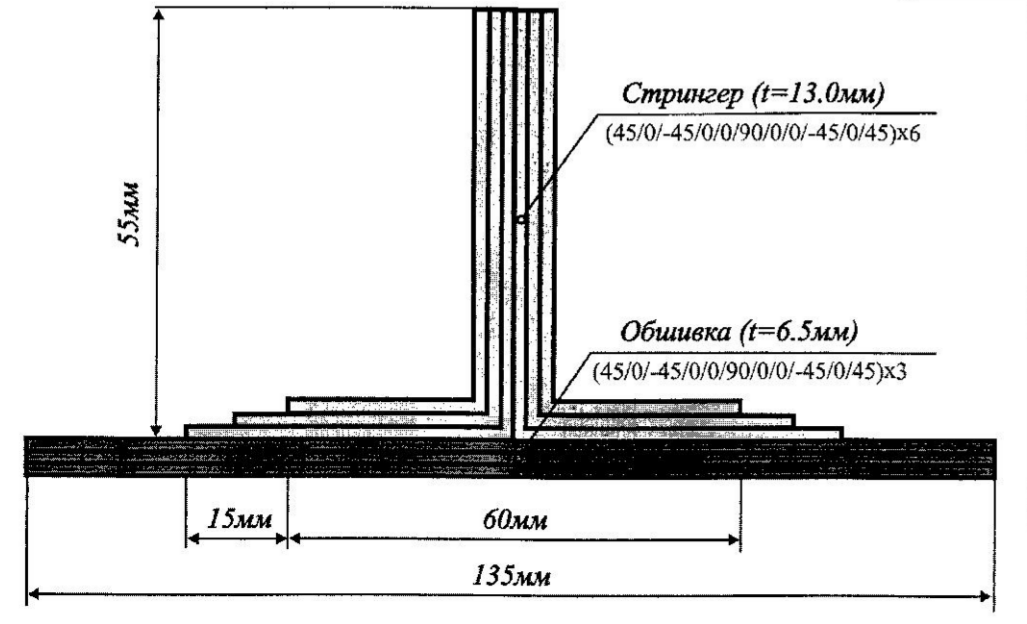
\includegraphics[width=\textwidth]{png/construction.png}}
\caption{Обшивка и силовой кессон крыла.}
\label{pic:construction}
\end{figure}
Одной из практических задач о динамическом нагружении композиционных материалов
является задача о непробивающем ударе по обшивке крыла самолёта. На рис.
\ref{pic:construction} приведена схема строения обшивки и силового кессона
крыла, выполненных из композиционных материалов. Обшивка толщиной 6.5 мм состоит 
из 3 композитных субпакетов, соединенных между собой эпоксидной смолой, 
а стрингер толщиной 13 мм -- из 6 аналогичных субпакетов. Каждый субпакет
состоит из 11 монослоёв со взаимной ориентацией субпакетов при укладке 
45/0/-45/0/0/90/0/0/-45/0/45. Каждый монослой имеет следующий состав: 60\% -- 
ориентированные длинные углепластиковые волокна; 40\% -- матрица
(эпоксидная смола). 

Ввиду большой вычислительной сложности при моделировании подобной конструкции с 
точностью до отдельного волокна, а также из-за многообразия протекающих процессов, 
полная задача декомпозируется на ряд подзадач. В данной работе рассматривается задача о получении
волновой картины в элементе композитной обшивки крыла при следующих условиях:
\begin{itemize}
\item обшивка состоит из трёх субпакетов, сооединённых эпоксидной смолой;
\item каждый субпакет изотропен по своим свойствам;
\item толщина субпакетов и соединяющих эпоксидных слоёв одинакова;
\item размеры одного субпакета: 20x20x1 мм.
\end{itemize}
Упругие характеристики слоёв приведены в табл. \ref{tbl:subpackage}
\begin{table}
\centering
\begin{tabular}{|c|c|c|c|c|c|c|c|}
\hline
Слой & E, ГПа & $\nu$ & $\rho$, кг/м$^{3}$ & $\lambda$, ГПа & $\mu$, ГПа &
$c_p$, м/с & $c_s$, м/с \\
\hline
Эпоксидная смола & 2.5 & 0.3 & 1250 & 1.44 & 0.96 & 1640 & 876 \\
Субпакет & 8 & 0.3 & 1250 & 4.62 & 3.08 & 2937 & 1570 \\
\hline
\end{tabular}
\caption{Упругие характеристики слоёв.}
\label{tbl:subpackage}
\end{table}
Эти параметры в изотропном приближении моделируют обшивку крыла самолёта и
позволяют качественно получить волновую картину после непробивающего удара.

В эксперименте по непробивающему воздействию на обшивку нагрузка создается 
металлическим ударником диаметром 25.4 мм. Характерный пример профиля нагрузки 
при испытаниях приведен на рис. \ref{pic:loadprofile}. Давление на поверхности 
крыла в ходе эксперимента находится в диапазоне 0-100 Мпа. Поэтому для численного 
моделирования выбирается воздействие с давлением 50 Мпа.
\begin{figure}[h]
\center{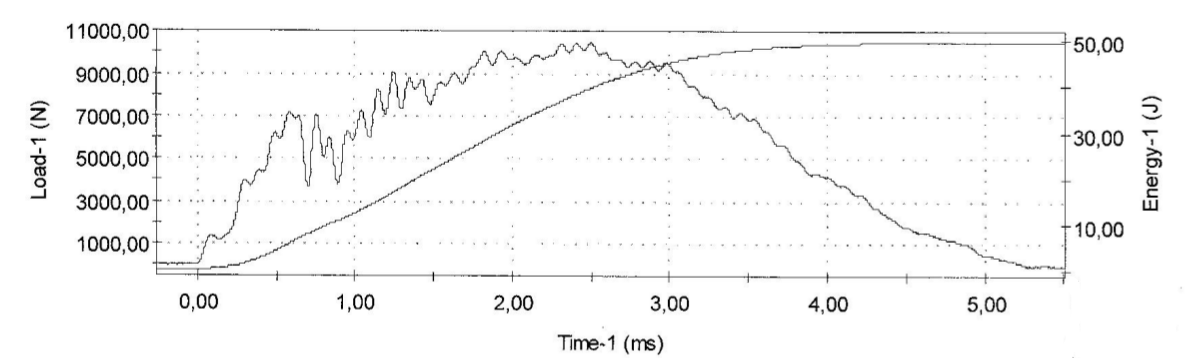
\includegraphics[width=\textwidth]{png/load-profile.png}}
\caption{Пример профиля нагрузки на обшивку крыла при испытаниях.}
\label{pic:loadprofile}
\end{figure}

Резюмируя, можно выделить следующие цели работы:
\begin{itemize}
\item предложить алгоритм построения параллельной версии сеточно"=характеристического метода в случае трёх пространственных переменных на неструктурированных сетках;
\item реализовать предложенный алгоритм в виде программного комплекса;
\item получить волновую картину в обшивке после низкоскоростного удара при
указаных выше допущениях.
\end{itemize}

\subsection*{Существующие работы на схожую тематику}
\addcontentsline{toc}{subsection}{Существующие работы на схожую тематику}

Для динамических задач механики деформируемого твердого тела необходимо использование численных методов, позволяющих получить полную волновую картину с высоким временным и пространственным разрешением с учётом влияния контактных границ. Так как определяющая система уравнений в частных производных относится к гиперболическому типу, одними из наиболее широко используемых вычислительных методов для её решения являются сеточно-характеристические методы, подробное описание и обзор которых можно найти в \cite{magomedov}. Главная особенность, присущая методу характеристик, -- нерегулярность разностной сетки -- оказалась серьёзным препятствием для обобщения этого метода на многомерный случай. Существенное продвижение здесь было получено в работах \cite{chushkin}, основанных на сочетании метода характеристик и конечно-разностных подходов.

В работе \cite{petrov_chelnokov} рассматриваются особенности протекания процессов деформирования в многослойных преградах конечной толщины, вызванных ударом абсолютно твёрдого сферического тела. Для моделирования поведения материала преграды использовались реологические модели линейно-упругой среды (закон Гука), упругопластической (модель Прандтля-Рейса с условиями пластичности Мизеса и Мизеса-Шлейхера, модель Маквелла), упруговязкопластической сред. Характерной особенностью работы является использование модели разрушения (модель Майнчена-Сака), а также использование различных подходов к перестроению сеток. Для численного решения использовался сеточно-характеристический метод, гибридная и гибридизованная разностные схемы. Минусами является использование структурированной (прямоугольной) сетки и только двух пространственных переменных.

В работе \cite{matyushev_petrov} проводилось численное исследование волновых и деформационных процессов в многослойных  средах. Как и в предыдущей работе, использовался численно-характеристический метод, а также гибридная и гибридизированная схемы. Особенностью является использование неструктурированных (треугольных) сеток, а также применение сеточно-характеристического шаблона на неструктурированных сетках (этот подход весьма необычен, так как использование шаблона предполагает наличие структурированной сетки). Моделировался удар деформируемым сферическим ударником по многослойной (5 – 20 слоев) преграде. Данная модель описывала пуленепробиваемый жилет и человеческое тело, защищённое им. Целью было найти оптимальные параметры среды для максимального поглощения воздействия ударника. К недостаткам работы можно отнести моделирование лишь по двум пространственным координатам.

В \cite{petrov_tormasov_holodov} рассматрены одномерные и двумерные нестационарные задачи о действии ударных и других нестационарных нагрузок на деформируемые твёрдые среды многослойной структуры, описаны возникающие волновые и откольные эффекты. Для описания поведения среды использованы модели линейно упругого и упругоидеальнопластического тела. На поверхностях раздела слоев рассматрены условия трёх типов: полного слипания, свободного скольжения, отслоения. В работе изучалось в основном влияние многослойных структур на амплитуду проходящей волны. На основании одномерных расчётов в слоистых средах был сделан вывод, что слоистые конструкции можно использовать для уменьшения амплитуды волн и для увеличения сжимающих напряжений вблизи лицевой поверхности, например, для увеличения силы сопротивления.

В \cite{golubev_kvasov_petrov} исследуются задачи распространения упругих волн, возникающих в результате землетрясения, в различных геологических средах: однородной, многослойной, градиентной, с трещиноватым пластом и карстовым образованием. Также проводится анализ воздействия упругих волн на поверхностные промышленные сооружения: здания и плотины. Проводится сравнение воздействия упругих волн на дневную поверхность для различных геологических сред. Качественно рассматривается влияние упругих волн на прочность поверхностных сооружений. В работе используется сеточно"=характеристический метод на треугольных сетках, контактные границы выделяются явно.

В \cite{agapov_belocerkovsky_petrov} сформулирована двумерная математическая модель механической реакции головы человека на ударные воздействия, описывающая пространственное распределение механических нагрузок на мозг (который в принципе является многослойной средой). Приведены некоторые результаты ее численного исследования с применением сеточно-характеристических методов на структурированных (прямоугольных) и неструктурированных (треугольных) сетках.

Работа \cite{petrov} посвящена численному исследованию волновых и откольных явлений, возникающих при импульсном нагружении двух- и четырехслойных упругопластических цилиндрических оболочек конечной толщины, подкрепленных с тыльной стороны ребрами жесткости. Используется динамическая система двумерных уравнений механики деформируемого тела и упруго идеально пластическая модель Прандтля-Рейсса. В работе показана возможность не только получать разрушенные зоны, но и отдельные трещины, зоны концентраций напряжений вблизи трещины и края откольной зоны, которая переходит в трещину, являющуюся самостоятельным источником нестационарных возмущений.

Автору неизвесты работы на схожую тематику, использующие сеточно-характеристический метод на неструктурированных сетках при трех пространственных переменных с явным выделением контактных границ.

